\documentclass[conference]{IEEEtran}
\usepackage{graphicx}
\usepackage{lipsum} % solo para generar texto de ejemplo
\usepackage[english]{babel}
%Includes "References" in the table of contents
\usepackage[nottoc]{tocbibind}

\begin{document}

\title{Análisis, visualización y predicción de Precios Airbnb}

\author{%
\IEEEauthorblockN{Martin Navarrete Villegas}
\IEEEauthorblockA{Facultad De Ciencias Fisicomatemáticas\\
Universidad Autónoma de Nuevo León\\
Correo electrónico: martin.nv6@gmail.com\\
Palabras clave: airbnb, prediccion, precio, nueva york, regresion.}
}

\maketitle

\begin{abstract}
En el presente documento se comparan los resultados obtenidos de la aplicacion de diversos modelos de regresion sobre datos referentes a hospedajes de la plataforma de airbnb en el area metropolitana de Nueva York, para tratar de encontrar una metodologia eficaz y con alta precision en la prediccion de precios por dia para hospedajes, esto basandosnos en diversas variables de las habitaciones.
\end{abstract}

% Keywords command
\providecommand{\keywords}[1]
{
  \small	
  \textbf{\textit{Keywords---}} #1
}
\keywords{airbnb, prediccion, precio, nueva york, regresion.}

\section{Introducción}
La era de la pandemia de covid nos obligo a cambiar nuestra forma de vivir, con ello la manera en la que viajamos y nos hospedamos cambio, Airbnb es un servicio de interenet que provee la plataforma para conectar propietarios de casas o departamentos con clientes potenciales, durante la pandemia esta plataforma alcanzo niveles de uso muy altos, se realizo una comparacion de exactitud de modelos de regresion para prediccion de precios de hospedajes en Airbnb basado en una serie de parametros como el tipo de habitacion, la cantidad de opiniones en el sitio, cantidad de dias de ocupacion y el barrio.

\subsection{Objetivo principal}
Realizar una comparacion de exactitud de modelos de regresion para prediccion de precios de hospedajes en Airbnb.
\subsection{Objetivo secundario}
 Con los resultados lograr encontrar un algoritmo de prediccion de precios que pueda ser utilizado para calcular precios y encontrar las variables mas determinantes.

\section{Antecedentes}


\section{Descripción de datos}


\section{Metodología}
En el siguiente diagrama se muestra la metodologia que se siguio para esta investigacion
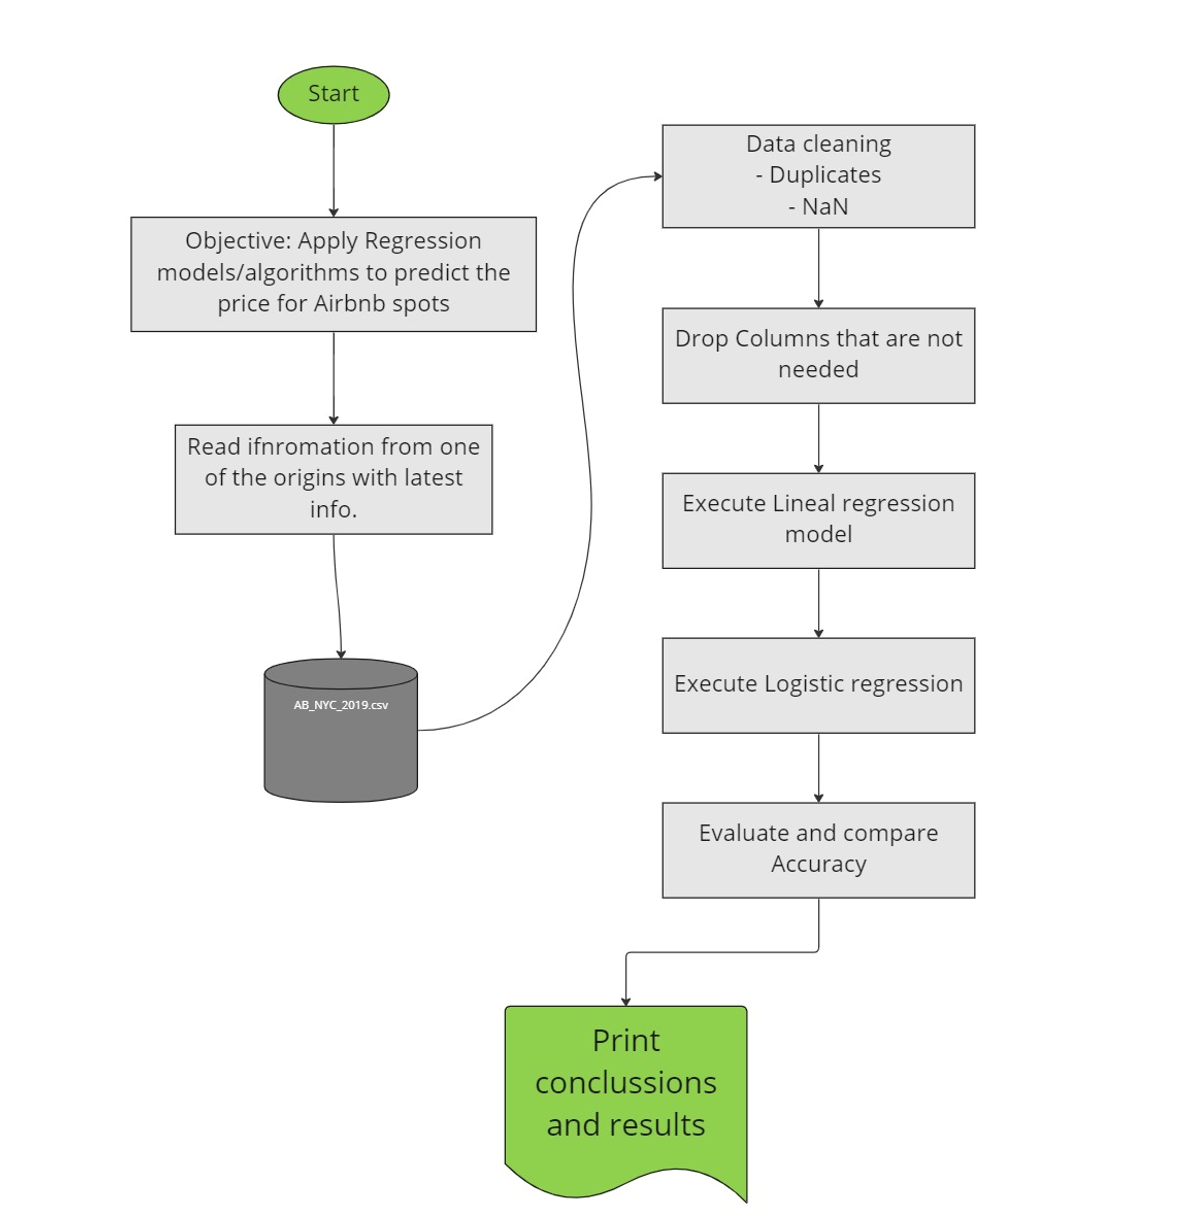
\includegraphics[width=10cm]{images/Metodologia.png}

Se comienza con lectura de los datos y con limpieza de estos, para ello se hace lo siguiente 
\begin{enumerate}
    \item Remover duplicados
    \item Revisar los valores nulos
    \item Reparar los valores nulos 
    \item En el caso de los valores nulos de 'reviewsPerMonth' se realiza un cambio de nulos por cero
    \item Algunos campos son eliminados como el 'hostid','latitude' y 'longitude'
\end{enumerate}

A continuacion se procedio con el analisis de regresion, en este caso se realizo usando Linear Regression y Decission tree regression.
\section{Resultados}


\section{Conclusiones}
\section{Trabajo a futuro}
Debido a que los resultados no fueron del todo satisfactorios en terminos de precision, como trabajo a futuro se realizara el procedimiento pero usando algoritmos de clasificacion, de esta manera quiza se logre un mejor resultados buscando precios "bajos", "medios" y "altos".
\vspace{5mm} %5mm vertical space

\bibliographystyle{ieeetr}
\bibliography{referencias} % aquí debes reemplazar "referencias" con el nombre de tu archivo .bib que contenga las referencias
\cite{Schwarzova_undated-cm,Schwarzova2020-ud,Kalehbasti2020-sk}
\end{document}